	\newpage
\section{Projektowanie}		%3
%Opis przygotowania narzędzi (git, visual studio). Wybór i opis bibliotek, klas. Szkic layoutów. Pseudo kody. Opisy wykorzystanych algorytmów (np. algorytm sortowania). Dokładniejsze określenie założeń i działania aplikacji, (np.: ten przycisk otworzy takie okno a w tym oknie wpisujemy takie dane).
\subsection{Android studio}

\hspace{0.60 cm}Podczas projektowania aplikacji mobilnej, użyliśmy przydatnego narzędzia jakm jest, Android Studio\cite{www1} version - Giraffe | 2022.3.1.
\begin{figure}[!hbt]
	\begin{center}
		
\includegraphics[width=\textwidth]{rys/giraffe.png}
		\caption{Android Studio Giraffe}
		\label{rys:Android-studio-Giraffe}
	\end{center}
\end{figure}

Będąc na stronie pobieramy aplikację przyciskiem "Download Android Studio Hedgehog".\textit{ (Android Studio to aplikacja ciągle się rozwijająca, więc możliwe jest że po wejściu na stronę Android Studio, przycisk pobierania pobierze nam aktualnie najnowszą wersję oprogramowania. Jeżeli chcielibyśmy wybrać konkretną wersję Android Studio, np: Giraffe/2022.3.1, musimy poszukać w wersjach archiwalnych. Tutaj znajduje się link do strony)}\cite{www2}.
	
Po przeczytaniu umowy licencyjnej, zaznaczamy przycisk i klikamy Download Android Studio. Po wskazaniu miejsca do instalacji, rozpocznie się proces pobierania.
\newpage
\begin{figure}[!hbt]
	\begin{center}
		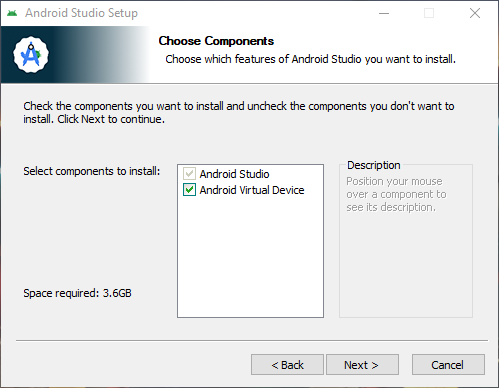
\includegraphics[width=10cm]{rys/InsAndr/1.png}
		\caption{Android Studio Instalacja}
		\label{rys:Android-studio-instalacja1}
	\end{center}
\end{figure}
W oknie instalatora, jako pierwsze ukażą się nam komponenty, które chcemy zainstalować wraz z narzędziem. W tym przypadku jesteśmy pytani czy chcemy aby obok aplikacji utworzyła się również domyślna wirtualna maszyna.

\begin{figure}[!hbt]
	\begin{center}
		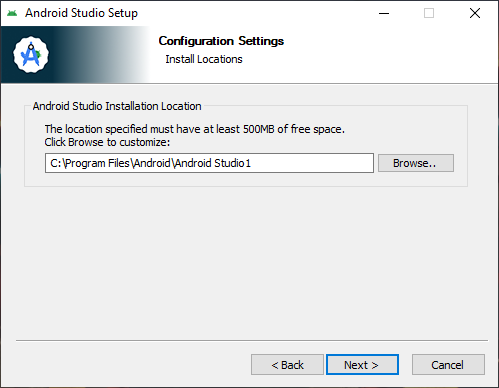
\includegraphics[width=10cm]{rys/InsAndr/2.png}
		\caption{Android Studio Instalacja}
		\label{rys:Android-studio-instalacja2}
	\end{center}
\end{figure}

Następnie wybieramy miejsce na dysku (przynajmniej 500MB wolnego miejsca), gdzie znajdować się będą nasze aplikacje. Klikamy "next", później "Install" i oczekujemy zakończenia procesu instalacyjnego.

\subsection{Github i Github Desktop}